This chapter provides a theoretical overview of the physics and mathematics this thesis is based on. First, we will define magnetic fields and provide a mathematical description. Then we will shortly discuss how magnetic fields can be measured, what the Earth's magnetic field is and how it can be approximated. Afterwards we give an introduction to quaternions and how they can be used to represent three-dimensional rotations. At the end, we introduce Bayesian statistics, which is related to particle filters.

\section{Magnetic fields}

A magnetic field is a vector field that describes the physical influence of moving electric charges and magnetic materials. Moving electric charges in a magnetic field experience a force perpendicular to their velocity and to the magnetic flux density, which is described by the Lorentz force. Additionally, the effects of the magnetic fields can be seen with permanent magnets which do not rely on macroscopic electrical currents. Permanent magnets attract or repel each other depending on their orientation and can pull on magnetic materials such as iron. The origin of macroscopic stationary magnetic fields are electrical currents and clusters of ordered magnetic moments of atoms. Magnetic moments of atoms are caused by orbital angular momentum of subatomic particles. Those are quantum mechanical effects and cannot be described by classical physics.

A magnetic field is only a part of the more general electromagnetic field. Since special relativity, we know that electric and magnetic fields can be transformed into each other by choosing different frames of reference.

In classical physics, electromagnetism has its foundation in the four microscopic Maxwell's equations and the Lorentz force. In SI units the equations are the following.\cite{demtroeder_mw}

\begin{equation}
\label{eq:maxwell_micro}
    \begin{aligned}[c]
        \nabla \cdot \bm{E} &= \frac{\rho}{\varepsilon_0}\\
        \nabla \times \bm{E} &= -\frac{\partial \bm{B}}{\partial t}\\
    \end{aligned}
    \qquad
    \begin{aligned}[c]
        \nabla \cdot \bm{B} &= 0\\
        \nabla \times \bm{B} &= \mu_0 \bm{J} + \mu_0 \varepsilon_0 \frac{\partial \bm{E}}{\partial t}\\
    \end{aligned}
\end{equation}

\begin{equation}
\label{eq:lorentz}
    \bm{F} = q\ (\bm{E} + \bm{v} \times \bm{B})
\end{equation}

The microscopic Maxwell Equations \ref{eq:maxwell_micro} are composed of the electric field strength vector $\bm{E}$, the magnetic flux density vector $\bm{B}$, the total electric charge density $\rho$, the total electrical current density vector $\bm{J}$, the permittivity of free space $\varepsilon_0$, and the permeability of free space $\mu_0$.

The Lorentz force $\bm{F}$ in Equation \ref{eq:lorentz} is the force acting on the charge $q$, that is moving with a velocity $\bm{v}$ through the electric field $\bm{E}$ and magnetic field $\bm{B}$.

Maxwell's equations are a set of coupled linear partial differential equations. Therefore the sum of two solutions yields another solution and the fields can be decomposed into the components of their origins.

There are two major variants of Maxwell's equations. The microscopic Maxwell Equations \ref{eq:maxwell_micro} have universal applicability in classical physics but are unpractical for analytical calculations and extensive numerical simulations. Solids contain approximately $10^{23}$ atoms per cm$^3$ which interact with each other, the bound electrons, and free electrons in case of a metal. The macroscopic Maxwell Equations \ref{eq:maxwell_macro} define two additional auxiliary fields (see Equations \ref{eq:maxwell_aux}) which describe the macroscopic response of the material to electromagnetic fields by neglecting microscopic structures and phenomena like atoms and spins. Their use requires material specific parameters which have to be measured experimentally or calculated with great numerical effort.\cite{demtroeder_mw}

\begin{equation}
\label{eq:maxwell_macro}
    \begin{aligned}[c]
        \nabla \cdot \bm{D} &= \rho_\text{f}\\
        \nabla \times \bm{E} &= -\frac{\partial \bm{B}}{\partial t}\\
    \end{aligned}
    \qquad
    \begin{aligned}[c]
        \nabla \cdot \bm{B} &= 0\\
        \nabla \times \bm{H} &= \bm{J}_\text{f} + \frac{\partial \bm{D}}{\partial t}\\
    \end{aligned}
\end{equation}

\begin{equation}
\label{eq:maxwell_aux}
    \begin{aligned}[c]
        \bm{D} &= \varepsilon_0 \bm{E} + \bm{P}\\
        \bm{H} &= \frac{1}{\mu_0} \bm{B} - \bm{M}\\
    \end{aligned}
\end{equation}

The macroscopic Maxwell Equations \ref{eq:maxwell_macro} are composed of the electric displacement field vector $\bm{D}$, the magnetizing field vector $\bm{H}$, the free electric charge density $\rho_\text{f}$, and the free electrical current density vector $\bm{J}_\text{f}$.

The auxiliary fields are defined in the Equations \ref{eq:maxwell_aux}. Where $\bm{P}$ is the polarization field and $\bm{M}$ is the magnetization field. $\bm{P}$ and $\bm{M}$ are material specific and describe the response to external $\bm{E}$ and $\bm{H}$ fields.

\section{Magnetometer}

A magnetometer is an instrument that measures the local strength, direction or relative change of the magnetic field. There are many different types of magnetometers which rely on different physical phenomena of magnetic fields. Examples for these effects are induction currents, linear force or torque experienced by a magnetic dipole in a magnetic field, and the Lorentz force. 

In recent years, magnetometers have been miniaturized to the extent that they can be built into integrated circuits at very low cost. In 2009, the price of three-axis magnetometers dipped below one US dollar per device and dropped rapidly.\cite{magnetometer_price} As \gls{mems}, magnetometers are increasingly used as miniaturized compasses in smartphones and other devices. Compensation for temperature, hard iron, and soft iron effects are necessary.\cite{magnetometers}

\subsection{Hall-effect sensor}

\begin{figure}[hbt!]
    \centering
    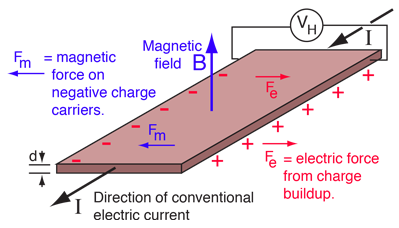
\includegraphics[width=0.5\textwidth]{figures/hall_effect.png}
    \caption{Schematic of a Hall probe measuring the magnetic field. Image gratefully taken from HyperPhysics.\cite{hyperphysics_hall_image}}
    \label{fig:hall_effect}
\end{figure}

The Hall-effect can be used to measure the magnitude of magnetic fields in one direction and is named after Edwin Hall who discovered it in 1879. As \gls{mems}, Hall-effect sensors are a popular alternative to magnetoresistive sensors.\cite{Hall1878}\cite{demtroeder_hall}

The effect is illustrated in Figure \ref{fig:hall_effect}. Magnetic fields exert a transverse force on moving charge carriers. This includes electrical currents in conductors. There, the magnetic field is pushing the charges to one side of the material which is most evident in thin flat conductors. The imbalance of the charges results in a measurable voltage between two sides of the conductor. Its output voltage $V_H$ is directly proportional to the magnetic field strength passing through the sensor, and is equal to:\cite{demtroeder_hall}

\begin{equation}
\label{eq:hall_effect}
    V_H = \frac{I B}{n e d}
\end{equation}

Where $I$ is the current flowing through the probe, $B$ is the magnetic field perpendicular to the probe, $n$ is the charge carrier density, $e$ the elementary charge, and $d$ is the probe thickness.

\section{Earth's magnetic field}
% TODO mention WWM2015 and their 12 harmonic approximation?

The Earth is sourcing a magnetic field from its interior which is reaching out into space, where it interacts with charged particles emitted by the Sun. The magnetic field is believed to be generated by electric currents in conductive convection streams of molten iron and nickel due to heat escaping the Earth's core. This process is complex and an active field of research. On the surface of the Earth, the magnitude of the magnetic flux density ranges from $25$ to $65$ $\mu$T. The field can be approximated by a magnetic dipole tilted at an angle of about $11$ degrees with respect to Earth's rotational axis.\cite{earth_magnetic_bible}\cite{earth_magnetic}

At any location, the Earth's magnetic field can be represented by a three dimensional vector. This is illustrated in Figure \ref{fig:earth_magnetic_field_coords}. A typical procedure for measuring its direction is to use a compass to determine the direction of magnetic North. Its angle relative to true North is called declination or variation. Facing magnetic North, the angle the magnetic field encloses with the horizontal plane is called inclination or magnetic dip. The intensity of the field is proportional to the force it exerts on a magnet. A common representation is X (North), Y (East) and Z (Down) coordinates.\cite{earth_magnetic}\cite{WWM2015}

\begin{figure}[hbt!]
    \centering
    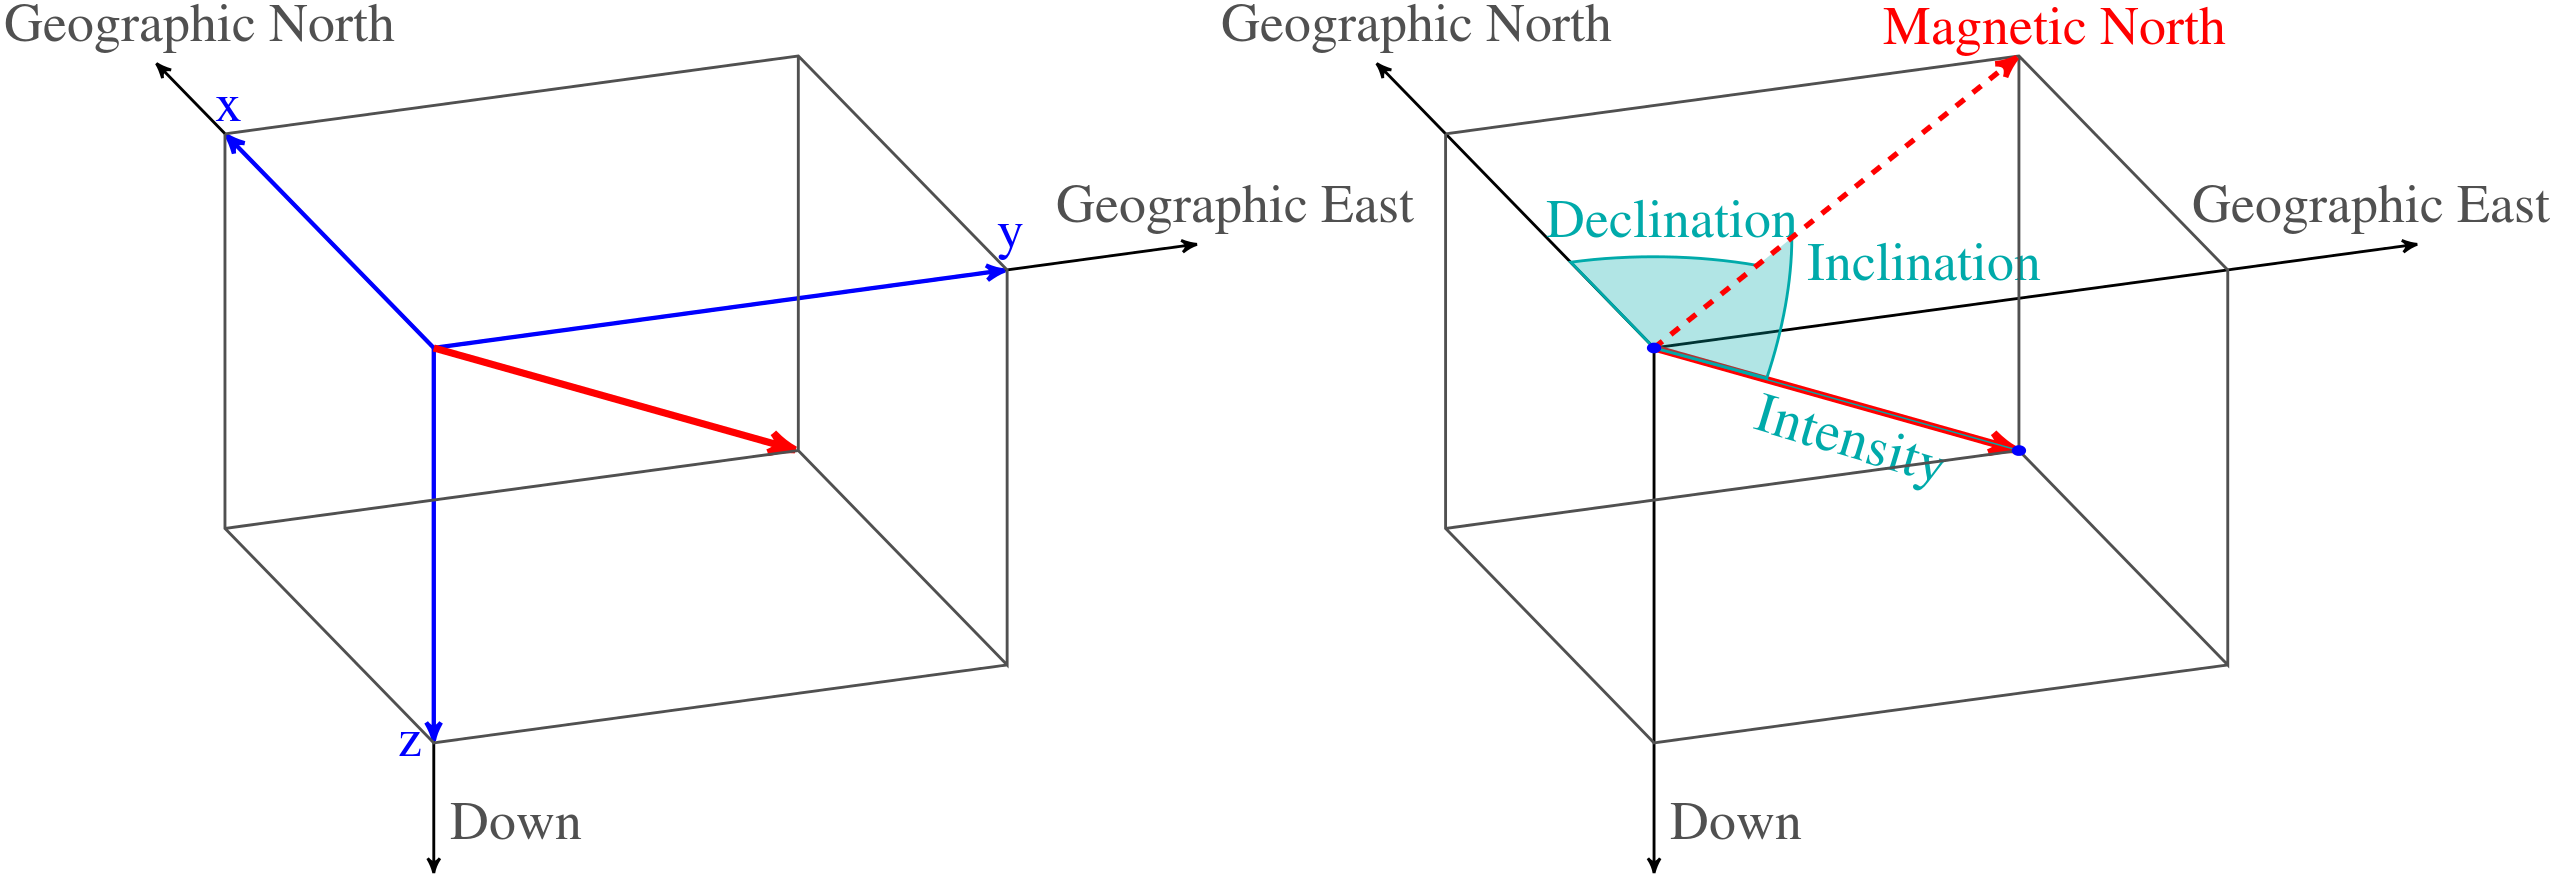
\includegraphics[width=1.0\textwidth]{figures/earth_magnetic_field_coords.png}
    \caption{Common coordinate systems used for representing the Earth's magnetic field. Image gracefully taken from Wikimedia.\cite{wikimedia_magcoords_image}}
    \label{fig:earth_magnetic_field_coords}
\end{figure}

\subsection{Dipole approximation}
\label{subsec:diple_approx}

In close proximity to the surface of the Earth, its magnetic field can be approximated by the field of a magnetic dipole placed at the center of the Earth and oriented with an angle of about $11$ degrees to the rotational axis of the Earth. In this description the Earth can be viewed as a strong bar magnet with its south pole pointing towards the geomagnetic North Pole. The dipole field accounts for approximately 80--90\% of the field in most locations.\cite{earth_magnetic}

In spherical coordinates, the dipole magnetic field of the Earth can be described as follows.\cite{earth_dipole}

\begin{equation}
\label{eq:dipole_approx}
    \begin{aligned}[c]
        B_r &= -2 B_0 ({\frac{R_E}{r}})^3 \cos \theta\\
        B_\theta &= - B_0 ({\frac{R_E}{r}})^3 \sin \theta\\
    \end{aligned}
\end{equation}

Where $B_0$ (typically $B_0 = 3.12*10^{-5}$ T) is the mean value of the magnetic flux density at the magnetic equator on the Earth's surface. $R_E$ is the mean radius of the Earth (approximately $6370\ \textrm{km}$), $r$ is the radial distance from the center of the Earth, and $\theta$ is the azimuth angle measured from the north geomagnetic pole.

This approximation is very practical for our purposes since it is easy to calculate the magnetic flux density for a given WGS84 position.

\section{Quaternions}
% TODO pauli matrices are a possible basis for quaternions
% TODO relation between pauli matrices, SU(2), SO(3)

Quaternions are a number system that extends the complex numbers with two additional imaginary axis. In 1843, they were described by the Irish mathematician William Rowan Hamilton and applied to mechanics in three-dimensional space.\cite{quaternions}

Quaternions are generally represented in the form

\begin{equation}
\label{eq:quaternion}
    \bm{q} = a + b \bm{i} + c \bm{j} + d \bm{k}
\end{equation}

where $a$, $b$, $c$, and $d$ are real numbers, and $\bm{i}$, $\bm{j}$, and $\bm{k}$ are the fundamental quaternion units, similar to the imaginary unit $\bm{i}$.

The imaginary units are connected through multiplication by

\begin{equation}
\label{eq:quaternion_units}
    \bm{i}^2 = \bm{j}^2 = \bm{k}^2 = \bm{ijk} = -1 \textrm{.}
\end{equation}

Quaternions are used in theoretical mathematics and applied mathematics. Applications are calculations involving three-dimensional rotations such as in computer graphics, computer vision, and crystallographic texture analysis. In practical applications, they can be used alongside other methods, such as Euler angles and rotation matrices, or as an alternative to them.

The unit quaternions can be thought of as a choice of a group structure on the 3-sphere $\text{S}^3$ that gives the group $\text{Spin}(3)$, which is isomorphic to $\text{SU}(2)$ and also to the universal cover of $\text{SO}(3)$.

The conjugate of $q$ is given by $q^* = a - b \bm{i} - c \bm{j} - d \bm{k}$.

The norm by $\lVert q\rVert = \sqrt{qq^*} = \sqrt{q^{*}q} = \sqrt{a^2 + b^2 + c^2 + d^2}$.

The inverse by $q^{-1} = \frac{q^*}{\lVert q\rVert ^2}$.

\subsection{Quaternions as rotations}
% TODO mention that a quaternion can be constructed from euler axis+angle?
% TODO mention that all rotations in 3D can be parameterized as euler axis+angle and therefore as quaternion?

To express a rotation of an angle $\theta$ counterclockwise around a unit vector $\bm{u} = u_x \bm{i} + u_y \bm{j} + u_z \bm{k}$ we compose a unit quaternion with the extended Euler's formula

\begin{equation}
\label{eq:euler_ext}
    \bm{q} = e^{{\frac{\theta}{2}}{\bm{u}}} = \cos{\frac{\theta}{2}} + \sin{\frac{\theta}{2} \bm{u}} \textrm{ .}
\end{equation}

In order to apply this rotation to a point $\bm{p} = p_x \bm{i} + p_y \bm{j} + p_z \bm{k}$ one has to compute

\begin{equation}
\label{eq:quaternion_rotation}
    \bm{p}' = \bm{q} \bm{p} \bm{q}^{-1} \textrm{ .}
\end{equation}

Such a rotation is illustrated in Figure \ref{fig:quaternion_rot}.

Rotations can be composed by multiplying quaternions and reversed with the inverse quaternion $\bm{q}^{-1}$.

\begin{figure}[hbt!]
    \centering
    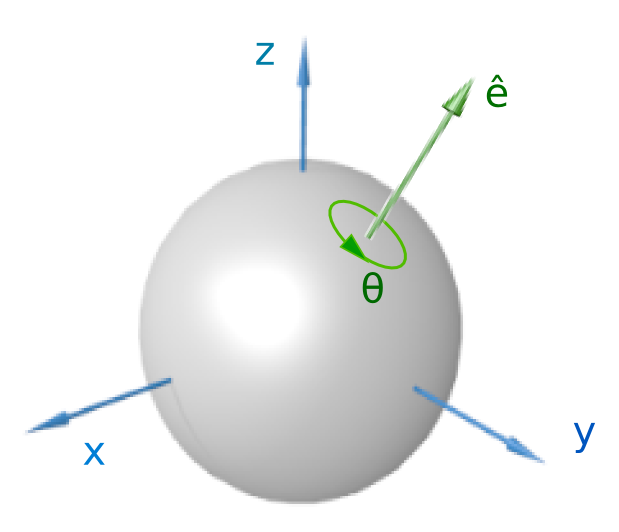
\includegraphics[width=0.5\textwidth]{figures/quaternion_rot.png}
    \caption{Illustration of a rotation represented by an Euler axis and angle. Image gracefully taken from Wikimedia.\cite{wikimedia_euleraxisangle_image}}
    \label{fig:quaternion_rot}
\end{figure}

\section{Bayesian statistics}
\label{sec:bayes}

Bayesian statistics is a theory based on the Bayesian interpretation of probability where it expresses a degree of belief in an event. The degree of belief can be based on prior knowledge about the event, like results of previous experiments, or on personal beliefs about the event. This differs from the frequentist interpretation which views probability as the limit of the relative frequency of an event after many trials.\cite{bayes_1}

Bayes' theorem is used in Bayesian methods to update probabilities after obtaining new data. Given two events $A$ and $B$, the conditional probability $P(A|B)$ -- the probability for $A$ given that $B$ is true -- is expressed as follows:\cite{bayes_1}

\begin{equation}
\label{eq:bayes}
    P(A|B) = \frac{P(B|A)\ P(A)}{P(B)} \textrm{  with  } P(B) \ne 0
\end{equation}

Bayes' theorem is a fundamental result of probability theory, but it has a specific interpretation in Bayesian statistics. In Equation \ref{eq:bayes}, $A$ represents a proposition (prior information like ``this coin lands on heads fifty percent of the time'') and $B$ represents new data we want to take into account (e.g. the result of a series of coin flips). $P(A)$ is the prior probability of $A$, which expresses our beliefs about $A$ before evidence is taken into account. $P(B|A)$ is the likelihood function, which can be interpreted as the probability of the evidence $B$ given that $A$ is true. The likelihood represents the model of the stochastic process and quantifies the extent to which evidence $B$ supports the proposition $A$. $P(A|B)$ is the posterior probability -- the probability of $A$ after taking the evidence $B$ into account. Essentially, Bayes' theorem updates our prior beliefs $P(A)$ after considering new evidence $B$.\cite{bayes_1}

In contrast to the frequentist interpretation, which views probability as the limit of the relative frequency of an event after many trials, Bayesian statistics does not rely on repeatable experiments. There is no true universal value of probability that we want to approach with many trials. Probability is a degree of belief based on data, a model and prior beliefs.
